% if you have a percent symbol, that line is commenting like in programming languages. it does not do anything.

% here, i specify the general style of the document. 
% you can play with it to see what changes, for example try removing twocolumn
\documentclass[aps,twocolumn,showpacs,preprintnumbers,nofootinbib,prl,superscriptaddress,groupedaddress]{revtex4-2}

% here are some "packages", basically utilities i need in this document. not all documents need all
% packages
\usepackage{amssymb,graphicx}
\usepackage{amsmath}
\usepackage{multirow}
\usepackage{epsfig}
\usepackage[usenames]{color} 
\usepackage[export]{adjustbox}
\usepackage{mathtools}
\usepackage{hyperref}

% you can define your own shortcuts etc, if you use sth very often
\newcommand{\balign}{\begin{align}}
\newcommand{\ealign}{\end{align}}

% or you can define your own symbols, check what this is
\def\meff{m_{\textrm{eff}}}


% here is where the document begins
\begin{document}

\title{LaTeX and Scientific Writing}
\author{Fethi M.\ Ramazano\u{g}lu} % turkish characters require special handling
\affiliation{Department of Physics, Ko\c{c} University, \\
Rumelifeneri Yolu, 34450 Sariyer, Istanbul, Turkey }
\date{\today}

\begin{abstract}
This document explains basics of Linux and scientific writing. It also serves
as a template for the term project in PHYS201: Classical Mechanics at Ko\c{c}
University. More information is given in the source file in terms of comments, 
which are also essential to understand LaTeX, so read this document together 
with the actual PDF output. It is prepared in the REVTeX-4.2 style, which is used by the 
journals published by the American Physical Society, some of the most
prestigious in the field (more specifically I use the PRL style).
This style is optimal for peer-reviewed publications
rather than term projects, but I wanted you to experience actual scientific
writing, so keep the document this way. This introductory part that gives
a short summary of a document is called the ``abstract'', and your project
should have one as well.
\end{abstract}
\maketitle


%%%%%%%%%%%%%%%%%%%%%%%%%%%%%%%%%%%%%%%%
\section{Beginning LaTeX}\label{intro}
%%%%%%%%%%%%%%%%%%%%%%%%%%%%%%%%%%%%%%%%
%%%%%%%%%%%%%%%%%%%%%%%%%%%%%%%%%%%%%%%%
LaTeX (stylized as \LaTeX) is a typesetting software commonly used by scientists to prepare manuscripts of various
kinds, mainly
peer-reviewed publications. You can use it for everyday purposes as well, it makes editing any
document very easy once you learn the basics. We are interested in writing a scientific project in this document.
LaTeX is pronounced as ``leytek'' in Turkish phonetics, the last letter is the Greek letter $\chi$, not a capital x.

% you get a new paragraph if you skip a line in the source file
To start with, go to the LaTeX project \href{https://www.latex-project.org/get/}{website}, download a LaTeX
distribution for your operating system and install it. I have a MacOS system, and use MacTeX.
Previously, I used MikTeX on Windows and TeX Live on Linux. Any of them (or some other up to date
version) would do.

Now, the distribution has all the files that is required to prepare a document, but you may still need an editor
to write the document. Some LaTeX distributions also come with an editor, some don't, and such editors may
not be the best. I prefer \href{https://pages.uoregon.edu/koch/texshop/}{TeXShop} on Mac, and previously
used \href{http://www.xm1math.net/texmaker/}{TeXMaker} on Linux, and
\href{http://www.winedt.com/}{WinEdt}\footnote{This one asks for donations after a while you use it, i remember 
uninstalling/installing it to stop the messages.} on Windows. I don't claim that these are superior in some way,
so make your own choice, but it is not a big deal as long as you don't dig up some obscure editor or
distribution.

There are also some online platforms which can be very useful for collaborative writing as is usual in scientific
publications. You may have a look at these if you are interested, but i advise to start with software on your own 
computer.

Once your software is in place, follow these steps:
\begin{itemize}
\item Open source.tex in your editor.

\item LaTeX the file. LaTeX is a command that makes your source file into a readable document.
For example, you do this by choosing the ``LaTeX'' command under the ``Typeset'' tab in TeXShop, your ediyor should
have a similar tab. This step is all to do for a most basic LaTeX document, ours is not so basic

\item From the same tab, execute the ``BibTeX'' command. This prepares your references as we detail below.
\item Run the ``LaTeX'' command \textbf{twice} more.

\item You should have the pdf version of this file generated in the folder. There are a bunch of other files as well, don't
worry about them.

\end{itemize}

%%%%%%%%%%%%%%%%%%%%%%%%%%%%%%%%%%%%%%%%
%%%%%%%%%%%%%%%%%%%%%%%%%%%%%%%%%%%%%%%%
\section{Some examples of scientific writing}
%%%%%%%%%%%%%%%%%%%%%%%%%%%%%%%%%%%%%%%%
%%%%%%%%%%%%%%%%%%%%%%%%%%%%%%%%%%%%%%%%
\subsection{Symbols}
I will just write some examples here, and you can see how it is done by looking at the source document. If you
need to write any symbol or short equation, for example the greek letter $\chi$, you put it between dollar signs
in the source file: $\$\textrm{chi}\$$. This is true for short equations as well: $\vec{F} = -\vec{\nabla}U$. Of
course you do not need to memorize all the special symbols, they are very very many, you look them up from
the web at first, and you learn the ones commonly used after a while (this is easier than it sounds).

If you have a long or major equation, you do not use the dollar signs, but specific ``environments`` such as
``equation'' or ``align''. Here is a single equation
\begin{equation}\label{lagrangian} 
% labels are basically tags for equations, see the text.
L = \frac{1}{2}m(\dot{r}^2+r^2\dot{\theta}^2)+ \frac{e^2}{r}-\frac{e}{2c}Br^2 \dot{\theta} \ ,
\end{equation}
and here is a few equations together
\begin{align}\label{coupled}
\ddot{x}_1 +\gamma \dot{x}_1+\omega_0^2 x_1 -\beta^2 x_2 &= 0 \nonumber \\
\ddot{x}_2 +\gamma \dot{x}_2+\omega_0^2 x_2 -\beta^2 x_1 &= 0 
% \nonumber forces that line to have no reference number
% the ampersand (&) is used to align the lines. the places you put them are at the same position in each line.
\end{align}
If you label your equations (see source), then you can reference them as Eq.~(\ref{lagrangian}) or Eq.~(\ref{coupled}).
Labelling is important, you should never refer to something with a number you write explicitly, since you always change
places of equations, add new ones, or delete some. By using labels, there is no need to rewrite the equation number,
you just look up its label (try erasing an equation, or adding another in between the ones above). Optionally, you can also put in-document links as in here, so that the reader can go to the relevant equation by clicking a number.

\subsection{Figures}
You can also easily add figures in LaTeX, such as Fig.~\ref{fig:rod_spring}. Note that by default you do not pick where
the figure ends up in the document, LaTeX takes care of it for you. If you want a specific place, there are ways to force
your will, but i would avoid that at this introductory level.
\begin{figure}
% figures can have labels as well
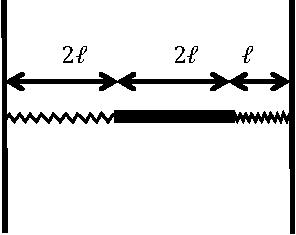
\includegraphics[width=0.35\textwidth]{rod_with_springs.pdf}
\caption{This is the explanation of the figure, called a ``caption''.}
\label{fig:rod_spring}
\end{figure}

\subsection{Citations and References}
Finally, a vital part of scientific publication is citing other publications, negligence in this regard is a grave offense, and
you should make it a habit to cite what you write if it comes from a specific source. \footnote{Of course, you do not
need to write the sources of common knowledge such as $F=ma$. Nevertheless, when in doubt, cite.} There are
various ways to arrange the references you cite, here i will show you how to use a .bib file using the command
``BibTeX''. There is a separate references.bib file in the same folder as the source.tex. This basically has the information
about all the sources you want to cite. Then, you just call their name with the ``cite'' command. For example PHYS201
textbook is~\cite{thornton2004classical}, or PHYS516 textbook is~\cite{Carroll:2004st}. Here is a citation to a
famous paper~\cite{Einstein:1905ve}. Of course, you do not cite documents like this, they come naturally in the text as in the following sentence:

``Einstein came up with the foundations of special relativity in 1905~\cite{Einstein:1905ve}.''

No one writes perfectly in the beginning, you learn the proper ways, and come up with your own style as you read and
write more papers.

You can put more than one source into a single reference as
in~\cite{thornton2004classical,Carroll:2004st,Einstein:1905ve}.

\textit{Acknowledgments:} I thank my students who made this class fun to teach, and all my teachers who taught me the 
wonders of classical mechanics.

\bibliography{references} % the name of the file where you keep the references you cite.

\end{document}
